\documentclass[en]{../../../eplsummary}

\usetikzlibrary{calc, trees, positioning, arrows, shapes, shapes.multipart, shadows, matrix, decorations.pathreplacing, decorations.pathmorphing}

\hypertitle{cloud-INGI2145}{7}{INGI}{2145}
{Houtain Nicolas, Thibault Gérondal}
{Canini Marco}

\section{Cloud computing}

\subsection{Introduction}

\begin{center}
\textit{Cloud computing is a model for enabling convenient, 
on-­demand network access to a shared pool of configurable 
computing resources (e.g., networks, servers, storage, 
applications, and services) that can be rapidly provisioned 
and released with minimal management effort or 
service provider interaction.}
\end{center}

\begin{tabular}{cm{10cm}}
    \textbf{Cloud commandments} &
\begin{enumerate}
    \item Partition everything
    \item Use asynchony everywhere
    \item Automate everything
    \item Remember that everything fails
    \item Embrace inconsistency
\end{enumerate}
\end{tabular}

\begin{tabular}{cm{10cm}}
    \textbf{Cloud benefit} &
\begin{itemize}
    \item Elastic,  just-­in-­time  infrastructure
    \item More  efficient  resource  utilization
    \item Pay  for  what  you  use
    \item Potential  to  reduce  processing  time (parallelization)
    \item Leverage  multiple  data  centers (high availability)
\end{itemize}
\end{tabular}


\subsubsection{Hardware scalability}

Cloud need for \textbf{scalability} because modern application require
huge amounts of processing and data. Cluster (\textit{room-sized}) and datacenter 
(\textit{building-sized}) can provide the resources needed.
They are composed of \textbf{rack} which is a aggregation of storage devices, many
nodes and switch to connect nodes together. Unfortunately, they are not perfect.
\begin{enumerate}
  \item Difficult to dimension because they must be provisioning for the peak load
  \item Expensive in hardware invest, expertise (ex: special software) and maintenance
  \item Difficult to scale because adding new machines is not easy
\end{enumerate}


\subsubsection{Model}
Cloud computing is a business models where everything is a service:
\begin{itemize}
  \item \textbf{SaaS}: Software as a service
  \item \textbf{PaaS}: Platform as a service
  \item \textbf{IaaS}: Infrastructure as a service
\end{itemize}

\subsubsection{Types}
There also have three types of cloud : 
\begin{itemize}
  \item \textbf{Public}: commercial commercial service open to almost anyone.
  \item \textbf{Community}: shared by several similar organization
  \item \textbf{Private}: shared within a organization
\end{itemize}
In this course we focus on public cloud.

\subsubsection{Applications}

Typically, applications that involve large amounts of computation, storage,
bandwidth Especially when lots of resources are needed quickly or load varies
rapidly.

\begin{itemize}
    \item \textbf{Web app}: Near the edge of the application focus is on vast 
    numbers of clients and rapid response
\item \textbf{Processing pipelines}: Inside we find data-­intensive services that 
    operate in a pipelined manner, asynchronously
  \item \textbf{Batch processing}: Deep inside the application we see a world of 
    virtual computer clusters that are scheduled to 
    share resources and on which applications like 
    MapReduce (Hadoop) are very popular
\end{itemize}


\subsubsection{Virtualization}
IS used to simulate multiple physical machine for the consumer with different
capabilities. It's powerful for security and isolation because VM cannot influence
other. In the other hand, performance is hard to predict because other VM run on
the same physical machine.

\subsubsection{Challenge}
\begin{tabular}{m{0.5\linewidth}m{0.5\linewidth}}
\begin{itemize}
  \item Availability
  \item Data lock-in (moving data)
  \item Data confidentiality and auditability 
  \item Data transfer bottlenecks
  \item Performance unpredictability for VM
\end{itemize}
&
\begin{itemize}
  \item Scalable storage
  \item Bugs in large distributed systems
  \item Scaling quickly
  \item Reputation fate sharing
  \item Software licensing
\end{itemize}
\end{tabular}


\section{Design for scale}

A system is scalable if it can easily adapt to 
increased (or reduced) demand.

\subsection{Parallelism programming}

\subsubsection{Vocabulary}
\begin{description}
  \item[Parallelism]: refers to techniques to make programs faster by
    performing several computations in parallel.

  \item[Concurrency]: is the composition of independently executing
    computations.
\end{description}

\subsubsection{Parallelization}
\begin{itemize}
  \item \textbf{Amdahl's law}:

    \begin{tabular}{m{0.5\linewidth}m{0.5\linewidth}}
    $$\quad S = \frac{1}{\alpha +
    \frac{1-\alpha}{N}}$$ where $\alpha$ is the sequential part and $N$ the
    number of cores.
    &
    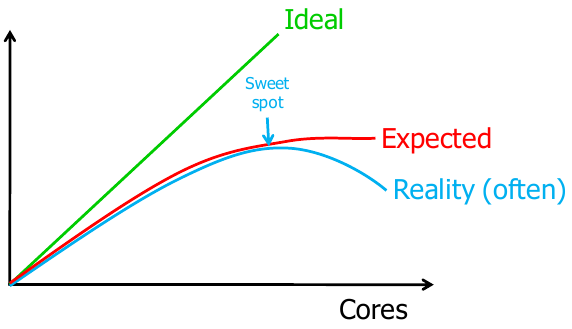
\includegraphics[width=6cm]{img/amdahl.png}
  \end{tabular}

  The coarse-grain (opposited to fine-grain) parallelism is more efficient
  because he limits the communication and coordination overheads by allow
  bigger task.
  \item \textbf{Dependencies}: Some task need to be after other which limits the degree of 
    parallelism. $\rightarrow$ Scheduling problem
\end{itemize}

\subsubsection{Architecture}
\begin{itemize}
  \item Symmetric multiprocessing (SMP): all processors share same memory.
    
    \begin{tabular}{m{0.7\linewidth}m{0.3\linewidth}}
      \begin{itemize} 
        \item[+] Simplicity and easy to load balance 
        \item[-] Scalability limited and expensive
      \end{itemize}
      &
        \begin{tiny}
      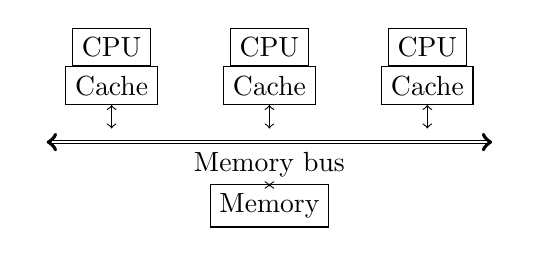
\begin{tikzpicture}
          \node[draw, rectangle] (1) {CPU};
          \node[draw, rectangle] (2) [right=of 1] {CPU};
          \node[draw, rectangle] (3) [right=of 2] {CPU};

          \node[draw, rectangle] (11) [below=0cm of 1] {Cache};
          \node[draw, rectangle] (21) [below=0cm of 2] {Cache};
          \node[draw, rectangle] (31) [below=0cm of 3] {Cache};

          \node (12) [below=0.3cm of 11] {};
          \node (22) [below=0.3cm of 21] {};
          \node (32) [below=0.3cm of 31] {};

          \node (tmp) [below left=  -0.2cm and 0.7cm of 12] {};
          \node (tmp2) [below right=-0.2cm and 0.7cm of 32] {};

          \draw (tmp) edge[double, <->] node[below](p) {Memory bus} (tmp2);
            \draw (12) edge[<->] (11);
            \draw (22) edge[<->] (21);
            \draw (32) edge[<->] (31);

          \node[draw, rectangle] (mem) [below=1.0cm of 21] {Memory};
            \draw (mem) edge[<->] (p);
      \end{tikzpicture}
        \end{tiny}
    \end{tabular}

  \item Non Uniform memory architecture (NUMA)
    
    \begin{tabular}{m{0.7\linewidth}m{0.3\linewidth}}
      \begin{itemize} 
        \item[+] Better scalability and faster memory
        \item[-] Complicates programming and scalability limited
      \end{itemize}
      &
        \begin{tiny}
      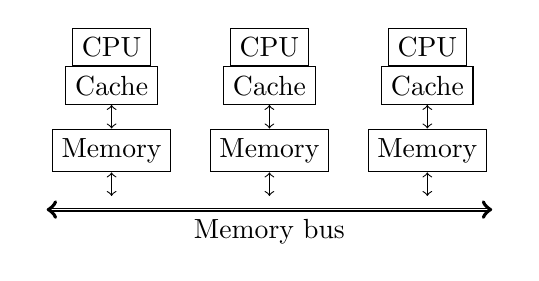
\begin{tikzpicture}
          \node[draw, rectangle] (1) {CPU};
          \node[draw, rectangle] (2) [right=of 1] {CPU};
          \node[draw, rectangle] (3) [right=of 2] {CPU};

          \node[draw, rectangle] (11) [below=0cm of 1] {Cache};
          \node[draw, rectangle] (21) [below=0cm of 2] {Cache};
          \node[draw, rectangle] (31) [below=0cm of 3] {Cache};

          \node[draw, rectangle] (12) [below=0.3cm of 11] {Memory};
          \node[draw, rectangle] (22) [below=0.3cm of 21] {Memory};
          \node[draw, rectangle] (32) [below=0.3cm of 31] {Memory};

          \node (13) [below=0.3cm of 12] {};
          \node (23) [below=0.3cm of 22] {};
          \node (33) [below=0.3cm of 32] {};

          \node (tmp) [below left=  -0.2cm and 0.7cm of 13] {};
          \node (tmp2) [below right=-0.2cm and 0.7cm of 33] {};

          \draw (tmp) edge[double, <->] node[below](p) {Memory bus} (tmp2);
            \draw (12) edge[<->] (11);
            \draw (22) edge[<->] (21);
            \draw (32) edge[<->] (31);

            \draw (12) edge[<->] (13);
            \draw (22) edge[<->] (23);
            \draw (32) edge[<->] (33);
      \end{tikzpicture}
        \end{tiny}
    \end{tabular}

  \item Shared Nothing
    
    \begin{tabular}{m{0.7\linewidth}m{0.3\linewidth}}
      \begin{itemize} 
        \item[+] Nice scalability
        \item[-] Requires different programming model
      \end{itemize}
      &

        \begin{tiny}
      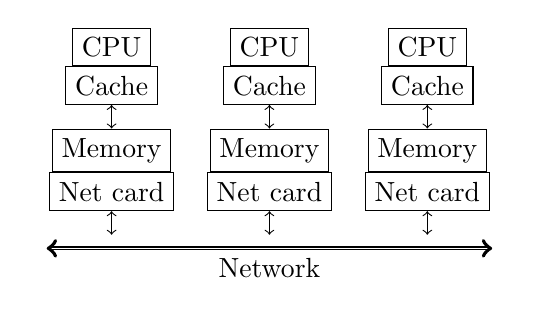
\begin{tikzpicture}
          \node[draw, rectangle] (1) {CPU};
          \node[draw, rectangle] (2) [right=of 1] {CPU};
          \node[draw, rectangle] (3) [right=of 2] {CPU};

          \node[draw, rectangle] (11) [below=0cm of 1] {Cache};
          \node[draw, rectangle] (21) [below=0cm of 2] {Cache};
          \node[draw, rectangle] (31) [below=0cm of 3] {Cache};

          \node[draw, rectangle] (12) [below=0.3cm of 11] {Memory};
          \node[draw, rectangle] (22) [below=0.3cm of 21] {Memory};
          \node[draw, rectangle] (32) [below=0.3cm of 31] {Memory};

          \node[draw, rectangle] (14) [below=0cm of 12] {Net card};
          \node[draw, rectangle] (24) [below=0cm of 22] {Net card};
          \node[draw, rectangle] (34) [below=0cm of 32] {Net card};

          \node (13) [below=0.3cm of 14] {};
          \node (23) [below=0.3cm of 24] {};
          \node (33) [below=0.3cm of 34] {};

          \node (tmp) [below left=  -0.2cm and 0.7cm of 13] {};
          \node (tmp2) [below right=-0.2cm and 0.7cm of 33] {};

          \draw (tmp) edge[double, <->] node[below](p) {Network} (tmp2);
            \draw (12) edge[<->] (11);
            \draw (22) edge[<->] (21);
            \draw (32) edge[<->] (31);

            \draw (13) edge[<->] (14);
            \draw (23) edge[<->] (24);
            \draw (33) edge[<->] (34);
      \end{tikzpicture}
        \end{tiny}
    \end{tabular}

\end{itemize}


\subsection{Distributed programming}

\subsubsection{Vocabulary}
\begin{description}
  \item[Faults]: Some component is not working correctly
  \item[Failure]: System as a whole is not working correctly
\end{description}

\subsubsection{Wide-area network}
The transfert speed for some data are defined by some attributs:
\begin{enumerate}
  \item Propagation delay
  \item Bottlenecks capacity on the path
  \item Queueing delay, loss, reordering, congestion, rtt 
    (take in account by TCP)
\end{enumerate}

$\rightarrow$ wide-area networks complicates the communication and faults are
more common

\subsubsection{Faults}

Fault are a common event in distributed system and some faults
are correlated.

\begin{itemize}
  \item \textbf{Crash faults}: node simply stop
  \item \textbf{Rational behavior}: owner manipulates node to increase profit
    (ex: lies on the routes to have traffic through it's own AS)
  \item \textbf{Byzantine faults}: faulty node could do anything (ex: stop, send spam,
    attack other, tell lies,...)
\end{itemize}

To prevent fault, we can \textit{prevent} them by using verification,
\textit{detect} them or \textit{mask} them by using replicas. The problem of
using \textbf{replicas} is to be able to maintain consistency between them!

\subsubsection{Consistency}

\begin{itemize}
  \item \textbf{Strong consistency}: After update completes, all subsequent
      accesses will return the updated value

  \item \textbf{Weak consistency}: After update completes, accesses do not
      necessarily return the updated value;; some condition must be satisfied
      first (such as update needs to reach all the replicas)

  \item \textbf{Eventual consistency}: Specific form of weak consistency: If no
      more updates are made to an object, then eventually all reads will return
      the latest value

  \item \textbf{Causal consistency}: If client A has communicated to client B that it
      has updated a data item, a subsequent access by B will return the updated
      value, and a write is guaranteed to supersede the earlier write. Client C
      that has no causal relationship to client A is subject to the normal
      eventual consistency rules

  \item \textbf{Read-your-writes consistency}:  Client A, after it has updated a data
      item, always accesses the updated value and will never see an older
      value.

  \item \textbf{Session consistency}: Like previous case but in the context of a
      session, for as long as the sessions remains alive.

  \item \textbf{Monotonic read consistency}: If client A has has seen a particular value
      for the object, any subsequent accesses will never return any previous
      values

  \item \textbf{Monotonic write consistency}: In this case the system guarantees to
      serialize the writes by the same process
\end{itemize}

We can combine them, and monotonic reads + read-your-write are most desirable
than eventual consistency.


\paragraph{Storage system example}


\begin{tabular}{m{5cm}m{12cm}}
    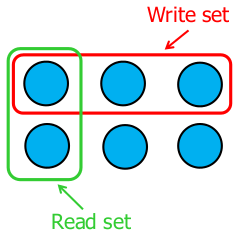
\includegraphics[width=3cm]{img/replicas} &
    
\includegraphics[width=7cm]{img/replicas2}
    \begin{itemize}
        \item[$\rightarrow$] Strong consistency
    \end{itemize} \\
\end{tabular}


\paragraph{Consensus}
\begin{enumerate}
    \item Clients send requests to each of the replicas
    \item Replicas coordinate and each return a result
    \item Client chooses one of the results, e.g., the one that is 
        returned by the largest number of replicas
    \item If a small fraction of the replicas returns the wrong result, or 
        no result at all, they are 'outvoted' by the other replicas
\end{enumerate}


\subsubsection{CAP theorem}
\begin{center}
    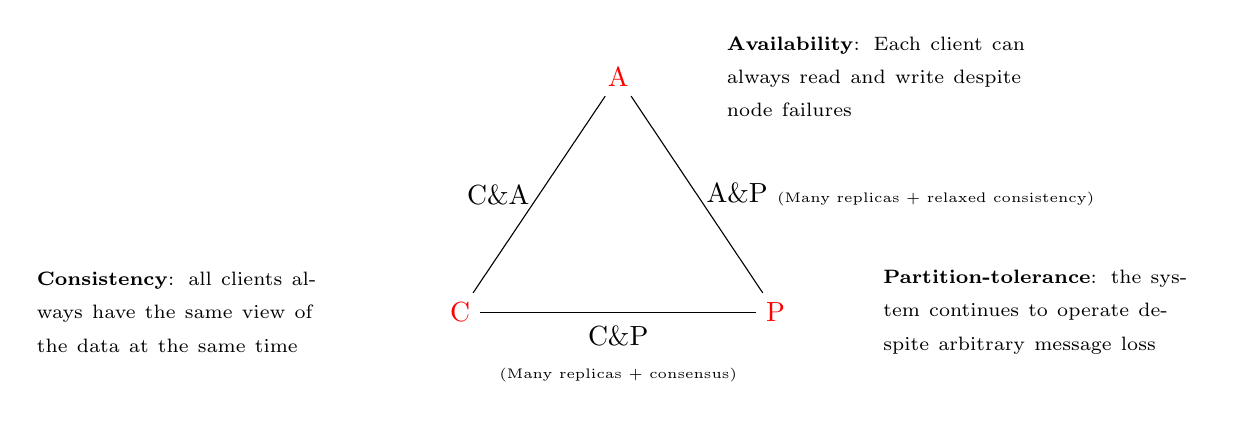
\begin{tikzpicture}
        \node (A) {\textcolor{red}{A}};
        \node (C) [below left=  2.5cm and 1.5cm of A] {\textcolor{red}{C}};
        \node (P) [below right= 2.5cm and 1.5cm of A] {\textcolor{red}{P}};

        \node[right =1cm of A, text width=4cm] {\scriptsize \textbf{Availability}: Each client can always read
        and write despite node failures};

        \node[left =1cm of C, text width=4cm] {\scriptsize \textbf{Consistency}: all clients always have the
        same view of the data at the same time};

        \node[right =1cm of P, text width=4cm] {\scriptsize \textbf{Partition-tolerance}: the
        system continues to operate despite arbitrary message loss};

        \draw (A) edge[-] node[left] {C\&A} (C);
        \draw (A) edge[-] node[right] {A\&P \tiny (Many replicas + relaxed consistency)} (P);
    \draw (C) edge[-] node[below] {\begin{tabular}{c}C\&P\\ \tiny (Many replicas + consensus) \end{tabular}} (P);
     \end{tikzpicture}
\end{center}


\paragraph{Actually}, we have a lot of partition and we have a trade-off
between C and A. \textbf{ACID} (atomicity, consistency, isolation, durability)
become \textbf{BASE} (basically available, soft-state, eventually consistent).


\subsection{Structure}
\begin{figure}[!h]
    \centering
    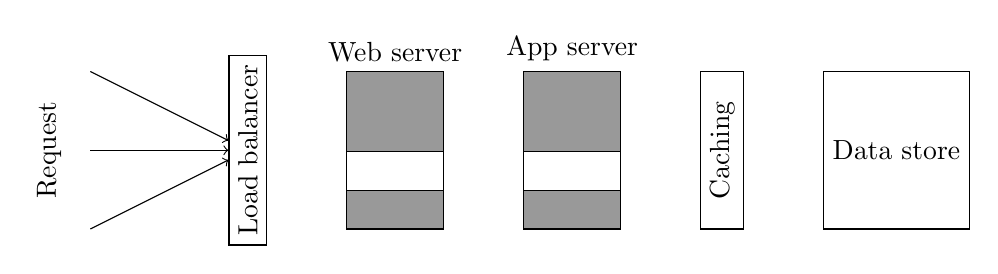
\begin{tikzpicture}

        \node[draw, rectangle, minimum height= 2cm] (L) {\rotatebox{90}{Load balancer}};
        \node[draw, rectangle, fill=black!40, minimum height= 2cm, text width=1cm, right= of L] (W) {};
        \node[draw, rectangle, fill= white, minimum height= 0.5cm, text width=1cm, below=-1cm of W] (W1) {};
        \node[above=0cm of W] (1) {Web server};

        \node[draw, rectangle, fill=black!40, minimum height= 2cm, text width=1cm, right= of W] (A) {};
        \node[draw, rectangle, fill=white,  minimum height= 0.5cm, text width=1cm, below=-1cm of A] (A1) {};
        \node[above=0cm of A] (1) {App server};

        \node[draw, rectangle, minimum height= 2cm, right= of A] (C) {\rotatebox{90}{Caching}};
        \node[draw, rectangle, minimum height= 2cm, right= of C] (D) {Data store};

        \draw[->] (-2, 0) -- (L);
        \draw[->] (-2, -1) -- (L);
        \draw[->] (-2, 1) -- (L);

        \node[left=2cm of L] (R) {\rotatebox{90}{Request}};

     \end{tikzpicture}
     \caption{Cloud structure with 
     caching which is  central  to  responsiveness}
\end{figure}

\begin{itemize}
    \item Stateless server: Views  a  client  request  as  an  independent  
        transaction  and  responds  to  it


        Easy to scale and more robuste because instance failure does not require
        overheas restoring state

    \item Statefull server: Scaling is challenging 
        
        \paragraph{Traditionnal approach is replication}
        \begin{itemize}
            \item Data  is  written  to  a  master  server  and  then  replicated  to  one  
        or  more  slave  servers  (synchronously  or  asynchronously))
            \item Read  operations  can  be  handled  by  the  slaves
        \end{itemize}

        But in this case, master becomes the write bottleneck and single point of failure.
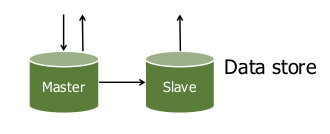
\includegraphics[width=5cm]{img/MasterSlave}

        \paragraph{Sharding with partitionning}
        Split  data  between  multiple  
        machines  and  have  a  way  to  make  sure  you  
        always  access  data  from  the  right  place. 
        Typically, define  a  sharding key  and  create  a  shard  mapping.

        Really high availability, incread read and write throughput and possibility 
        of doing more work in parallel within the application server.
        But the challenge is to find a good partitionning scheme.


        \subparagraph{} Sharging is  not  only  for  partitioning  data  
        within  a  database, but can be use to  partition  data  across  caching  
        servers (memcached, redis).
\end{itemize}

\paragraph{First-tier parallelism}
Parallelism  is  vital  for  fast  interactive  services, and 
parallel actions must focus on the critical path (it means delay that
contribute to the response delay and not asynchronous that are shortly)

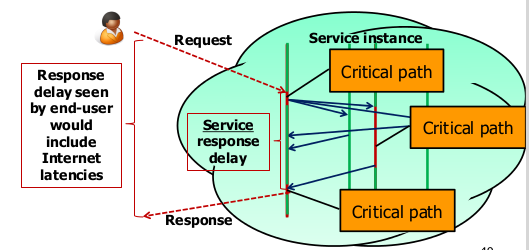
\includegraphics[width=5cm]{img/critical}


Note that update for replicas are typically done in asynchronous way, so we
might  not  experience  much  delay  on  the  critical  path.

Asynchronous  operations  decouple  systems  and  
enable  quicker  responses  at  the  expense  strong  
consistency.
Indeed, this can rise some issues which result in inconsistency:
\begin{itemize}
    \item We don't know in which order replicas applying the update
    \item The leader can crash before replicas change and lose some
        update
\end{itemize}


\section{Cloud storage}

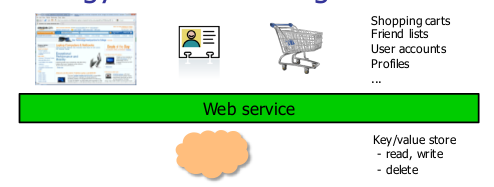
\includegraphics[width=5cm]{img/storage}
Many  cloud  services  have  a  similar  structure, 
But  the  actual  storage  service  is  very  simple (Read/write  'blocks',
similar  to  a  giant  hard  disk) and the translation  done  by  the  web  service.

\paragraph{ideal store}
\begin{itemize}
\item Perfect  durability – nothing  would  ever  disappear  in  a  crash
\item 100\%  availability – we  could  always  get  to  the  service
\item Zero  latency from  anywhere  on  earth  – no  delays!
\item Minimal  bandwidth  utilization  – we  only  send  across  the  network  what  we  absolutely  need
\item Isolation under  concurrent  updates  – make  sure  data  stays   consistent
\end{itemize}

BUT he  “cloud”  exists  over  a  physical  network (communication take time + limited bandwith)
and The  “cloud”  has  imperfect  hardware (failures)

\paragraph{Observation}
\begin{itemize}
    \item Read-­only  (or  read-­mostly)  data  is  easiest  to  support
    \item Granularity  matters:  “Few  large-­object”  tasks  generally  
        tolerate  longer  latencies  than  “many  small-­object”  tasks


        But  it’s  much  more  expensive to  replicate  or  to  update!

    \item[->] Maybe  it  makes  sense  to  develop  separate  solutions  for  large  
        read-­mostly  objects  vs.  small  read-­write  objects!
        Different  requirements  → different  technical  solutions
\end{itemize}


\subsection{Key-value stores (KVS)}
The  key-­value  store  (KVS)  is  a  simple  
abstraction  for  managing  persistent  state where data is 
organized  as  (key,value)  pairs with three basic operation:
\begin{enumerate}
    \item \texttt{PUT(key, value)}
    \item \texttt{value = GET(key)}
    \item \texttt{DEL(key)}
\end{enumerate}

\paragraph{Concurrency control}
Most  systems  use  locks on  individual  items.



\subsubsection{Amazon dynamo}
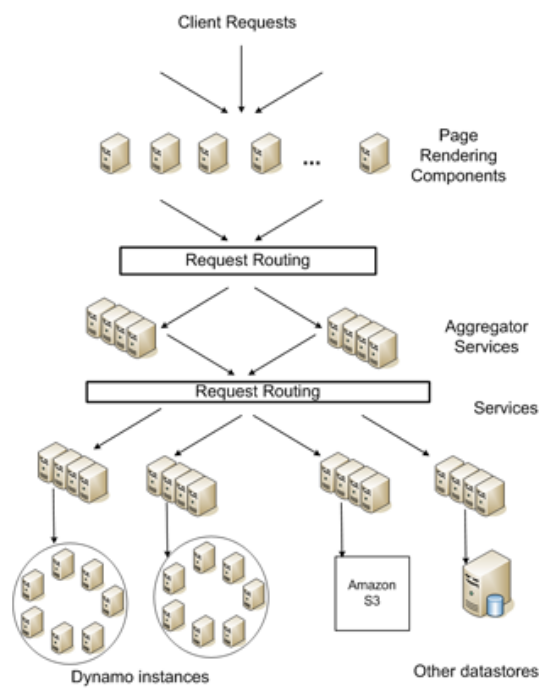
\includegraphics[width=5cm]{img/AWSplat}

AWS is AP and follow BASE philosophy. Dynamo is :
\begin{itemize}
    \item High performance with low latency
    \item High scalable
    \item High available key storage, especially for writes
    \item Partition/fault-tolerant
    \item Eventually consistent (sacrify for high availability)
\end{itemize}

Very  low  latency  writes,  reconciliation  in  reads.

\paragraph{Techniques}
\begin{itemize}
    \item \textbf{Consistent hashing}: dynamically partitions a set of  keys
        over  a  set  of  storage nodes (hash keys and give 
        a key of m-bits). One  key  range  per  virtual  node.

        \paragraph{Data partitioning and load balancing}
        A  key  is  assigned  to  the  closest   successor  node id 
        ( key  k  is  assigned  to  the  first  node  with  id  ≥ k )

        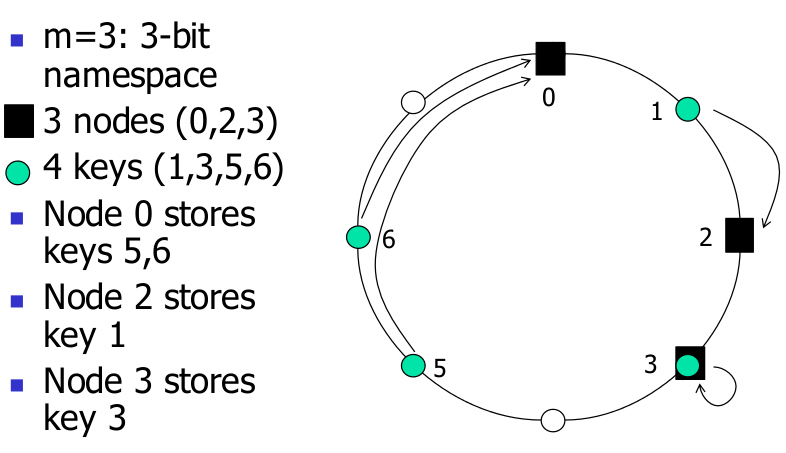
\includegraphics[width=5cm]{img/consistent}
        
        \begin{center}
            Each node has at most $(1+\epsilon) \frac{K}{N}$ keys with $N$ nodes, $K$ keys
            and $\epsilon=O(log(N))$
            %TODO: why epsilon=0 with virtual nodes?
        \end{center}

        \paragraph{Replication}
        Replication is done on the successors node because if the node fail, it's the successor
        which will take failed node keys.
        
        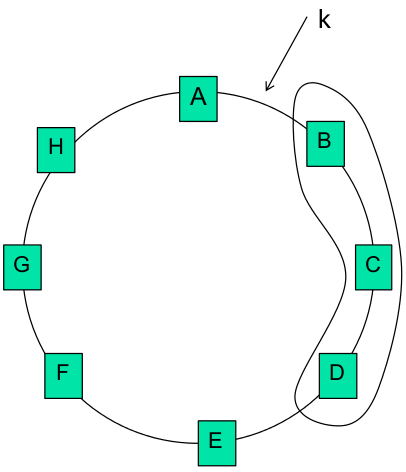
\includegraphics[width=5cm]{img/dynamoReplica}

        Replication is may in asynchronous way (eventual consistency), and
        key data versioning technique is done with vector clocks.


        If the replica A in  the  preference  list  is  down  then
        another  replica  is  created  on  a  new  node.
        In this case, coordinator  will  involve  D that substitutes
        A  until  A  comes  back  again. When  D  gets  info  A  is
        back  up it  hands  back  the  data  to  A


    \item \textbf{Vector clocks}: Each write  to  a  key  k  is  associated  with  a  
        vector  clock  VC(k) which is an  array  (map)  of  integers (one  entry  VC(k)[i]  for  each  node  i).

        This is use for  tracking  causal  dependencies  among  different  versions  
        of  the  same  key  (data)

        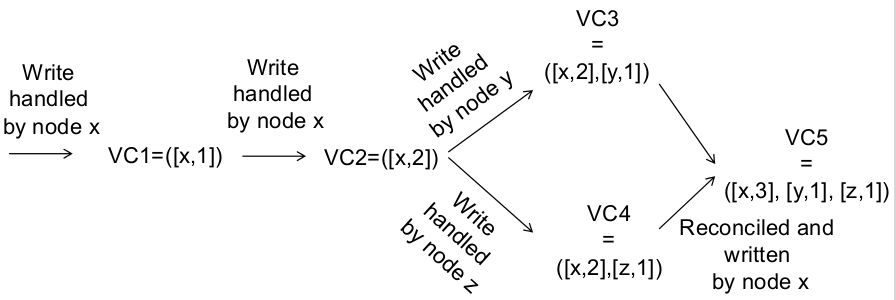
\includegraphics[width=5cm]{img/vectorClock}

    \item \textbf{Sloppy quorums}: In order to enforce consistency, to response
        to a read or write operation the node must asl to a \textit{quorum}
        which is the minimum number of votes that a distributed transaction has
        to obtain.

        \begin{itemize}
            \item $R$ number of nodes that participate in a get, $W$ number
                of node that participate in a write and $R+W > N$

            \item \textbf{Put}: Generate new $VC$, write locally, send value $VC$
                to N selected nodes from preference list and wait for $W-1$

            \item \textbf{Get}: Send read to $N$ selected nodes from preference list, 
                wait for $R$, select highest versions per $VC$ and return
                all such versions. 

                Writeback merge versions.

            \item[Note]
                \begin{enumerate}
                    \item Note that each node has routing info to all other node
                        to reduce latency (but this is lower scalable)
                        %TODO: slide 99 for 03
            \end{enumerate}
        \end{itemize}

        \textbf{Sloppy} allow  availability  under  a  much  wider  range  of  
        partitions  (failures)  but  sacrifice  consistency. The
        N  selected  nodes  are  the  first  N  healthy  
        nodes.

    \item \textbf{Anti-entropy protocol using hash/merkle tree}:
        Each  Dynamo  node  keeps  a  Merkle tree  for  
        each  of  its  key  ranges. Hash trees can be used to verify any kind of data stored.

        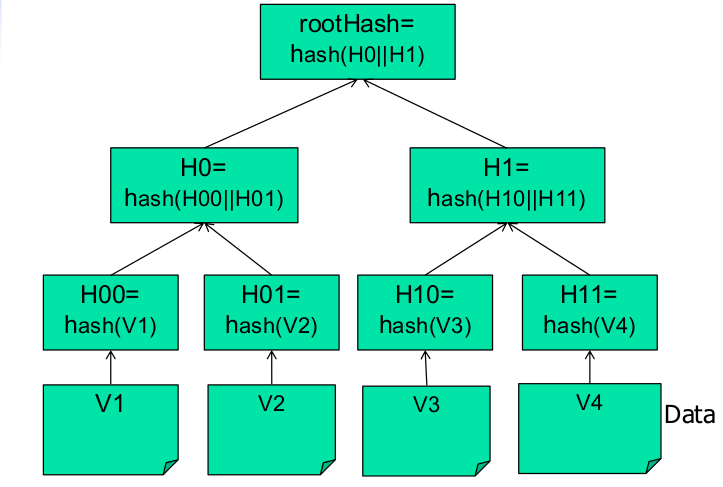
\includegraphics[width=5cm]{img/merkle}

        Compares  the  root  of  the  tree  with  replicas
        \begin{itemize}
            \item If  equal,  all  keys  in  a  range  are  equal  (replicas  in  sync)
            \item If  not  equal  
        Traverse  the  branches  of  the  tree  to  pinpoint  the  children  that  differ
        The  process  continues  to  all  leaves
        Synchronize  on  those  keys  that  differ
        \end{itemize}

    \item \textbf{Gossip-based group membership protocol}: 
        %TODO slides 106 for 03


        Membership  info  are  also  eventually  
        consistent  — propagated  by  background  
        gossip  protocol.
        \begin{itemize}
            \item Node  contacts  a  random  node  every  1s
            \item 2  nodes  reconcile  the  membership  info and partitioning/placement
                metadata
        \end{itemize}


        \paragraph{Unreliable failure detection (FD)}
        Used to  refresh  the  healthy  node  info  in  the  extended  
        preference  list.

        %TODO 107 for 03

\end{itemize}


\section{Paper}




\section{Summary of Eventually Consistent}

Data inconsistency in large-scale reliable distributed systems has to be tolerated for two reasons: improving read and write performance under highly concurrent conditions; and handling partition cases where a majority model would render part of the system unavailable even though the nodes are up and running.

Whether or not inconsistencies are acceptable depends on the client application. In all cases the developer needs to be aware that consistency guarantees are provided by the storage systems and need to be taken into account when developing applications.

\begin{description}
\item[Strong consistency] After the update completes, any subsequent access (by A, B, or C) will return the updated value.

\item[Weak consistency] The system does not guarantee that subsequent accesses will return the updated value. A number of conditions need to be met before the value will be returned. The period between the update and the moment when it is guaranteed that any observer will always see the updated value is dubbed the inconsistency window.

\item[Eventual consistency] This is a specific form of weak consistency; the storage system guarantees that if no new updates are made to the object, eventually all accesses will return the last updated value. If no failures occur, the maximum size of the inconsistency window can be determined based on factors such as communication delays, the load on the system, and the number of replicas involved in the replication scheme. The most popular system that implements eventual consistency is DNS (Domain Name System). Updates to a name are distributed according to a configured pattern and in combination with time-controlled caches; eventually, all clients will see the update.

\item[The eventual consistency has a number of variations that are important to consider:]

\item[Causal consistency] If process A has communicated to process B that it has updated a data item, a subsequent access by process B will return the updated value, and a write is guaranteed to supersede the earlier write. Access by process C that has no causal relationship to process A is subject to the normal eventual consistency rules.

\item[Read-your-writes consistency] This is an important model where process A, after it has updated a data item, always accesses the updated value and will never see an older value. This is a special case of the causal consistency model.

\item[Session consistency] This is a practical version of the previous model, where a process accesses the storage system in the context of a session. As long as the session exists, the system guarantees read-your-writes consistency. If the session terminates because of a certain failure scenario, a new session needs to be created and the guarantees do not overlap the sessions.

\item[Monotonic read consistency] If a process has seen a particular value for the object, any subsequent accesses will never return any previous values.

\item[Monotonic write consistency] In this case the system guarantees to serialize the writes by the same process. Systems that do not guarantee this level of consistency are notoriously hard to program.

\end{description}

A number of these properties can be combined. For example, one can get monotonic reads combined with session-level consistency. From a practical point of view these two properties (monotonic reads and read-your-writes) are most desirable in an eventual consistency system, but not always required. These two properties make it simpler for developers to build applications, while allowing the storage system to relax consistency and provide high availability.

\section{Course : Design for scale }

\subsection{Parallelism}

Assumption : All cores can access the same memory. Access latencies are uniform.

Problem :
\begin{itemize}
\item Difficult – need to find something for the other cores to do
\item Not all algorithms are equally parallelizable
\item Scalability. Usually, not all parts of the algorithm can be parallelized.
\end{itemize}

Increasing parallelism beyond a certain point can cause performance to decrease! Why?

\begin{itemize}
\item Time for serial parts can depend on \#cores
\item Need to send a message to each core to tell it what to do
\end{itemize}

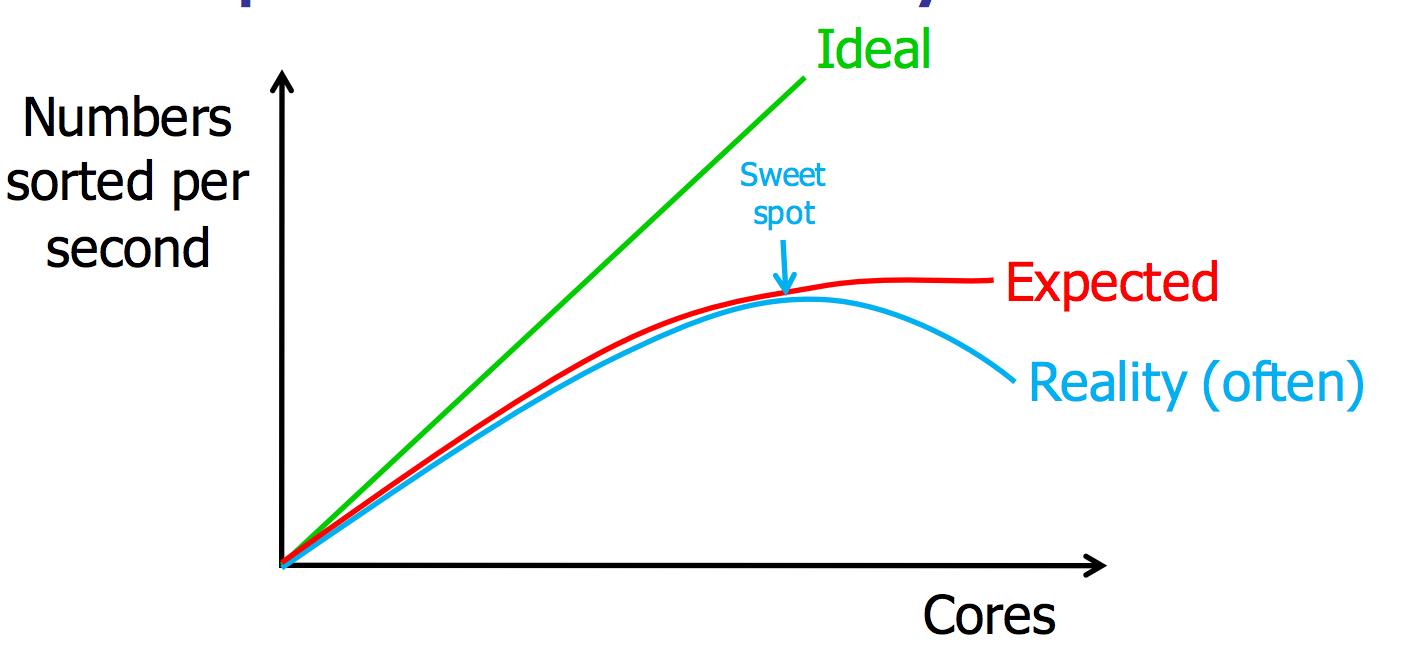
\includegraphics[width=\linewidth]{parall.png}

This graphic shows the Amdahl's law which gives the theoretical speedup in latency of the execution of a task at fixed workload that can be expected of a system whose resources are improved. It depends from parallelizable portion of the program.

\subsubsection{Coarse-grain vs. fine-grain parallelism}

Coarse-grain (gros grain) is better, less coordination messages (less overhead).


\subsubsection{Dependencies}

Dependencies : if tasks depend on other tasks => Limits the degree of parallelism. Minimum completion time (and thus maximum speedup) is determined by the longest path from start to finish. 

\subsubsection{Heterogeneity}

Heterogeneity : if tasks are harder than others or not all cores are equally fast. => Result: Scheduling problem (can be hard to solve).

\subsection{Parallelism vs Concurrency}

Parallelism refers to techniques to make programs faster by performing several computations in parallel (multi-core processors, compute clusters)

Concurrency is the composition of independently executing computations (It is a way to structure software and make it more usable)

\subsubsection{Race condition}

Result of the computation depends on the exact timing of the two threads of execution, i.e., the order in which the instructions are executed. Concurrent updates to the same state. 

\subsubsection{Goal: Consistency}

\begin{description}
\item[Sequential consistency] The result of any execution is the same as if the operations of all the cores had been executed in some sequential order, and the operations of each individual processor appear in this sequence in the order specified by the program.

\item[Strong consistency] After update completes, all subsequent accesses will return the updated value.

\item[Weak consistency] After update completes, accesses do not necessarily return the updated value; some condition must be satisfied first

\item[Eventual consistency] Specific form of weak consistency: If no more updates are made to an object, then eventually all reads will return the latest value

\item[Eventual consistency: Causal consistency] If client A has communicated to client B that it has updated a data item, a subsequent access by B will return the updated value, and a write is guaranteed to supersede the earlier write. Client C that has no causal relationship to client A is subject to the normal eventual consistency rules.

\item[Eventual consistency: Read-your-writes consistency] Client A, after it has updated a data item, always accesses the updated value and will never see an older value.

\item[Eventual consistency: Session consistency] Like previous case but in the context of a session, for as long as the sessions remains alive.

\item[Eventual consistency: Monotonic read consistency] If client A has has seen a particular value for the object, any subsequent accesses will never return any previous values.

\item[Eventual consistency: Monotonic write consistency] In this case the system guarantees to serialize the writes by the same process. Systems that do not guarantee this level of consistency are notoriously hard to program.

\item[Few consistency properties can be combined] monotonic reads + read-your-writes most desirable for eventual consistency.
\end{description}

\subsection{Architectures}
\subsubsection{Symmetric Multiprocessing (SMP)}
All processors share the same memory. Any CPU can access any byte; latency is always the same. Pros: Simplicity, easy load balancing. Cons: Limited scalability (~12 processors), expensive.

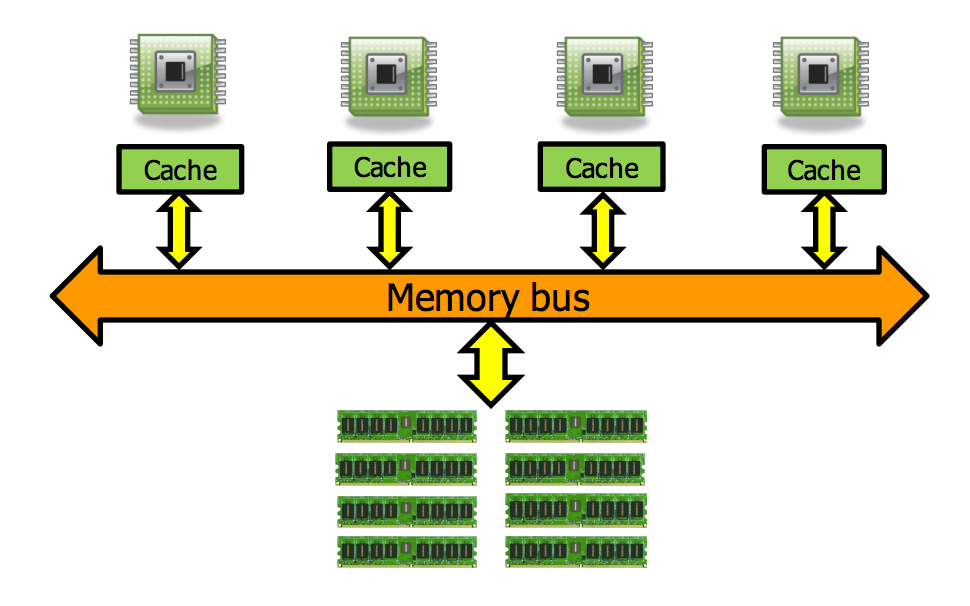
\includegraphics[width=\linewidth]{smp.png}

\subsubsection{Non-Uniform Memory Architecture (NUMA)}
Memory is local to a specific processor. Each CPU can still access any byte, but accesses to 'local' memory are considerably faster (2-3x). Pros: Better scalability. Cons: Complicates programming a bit, scalability still limited. 

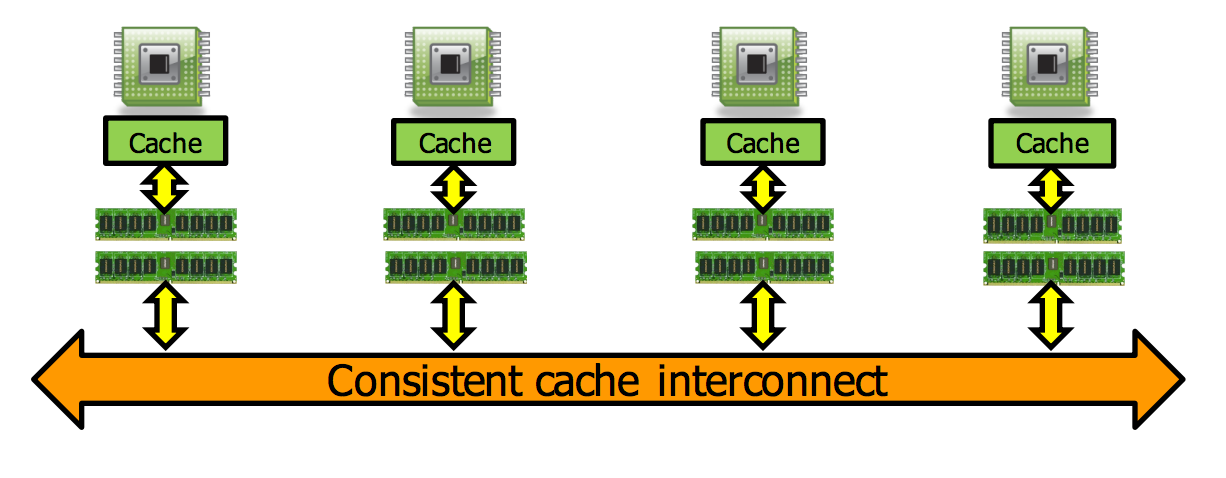
\includegraphics[width=\linewidth]{numa.png}

\subsubsection{Shared-Nothing}

Independent machines connected by network. Each CPU can only access its local memory; if it needs data from a remote machine, it must send a message there. Pros: Much better scalability. Cons: Requires a different programming model. 

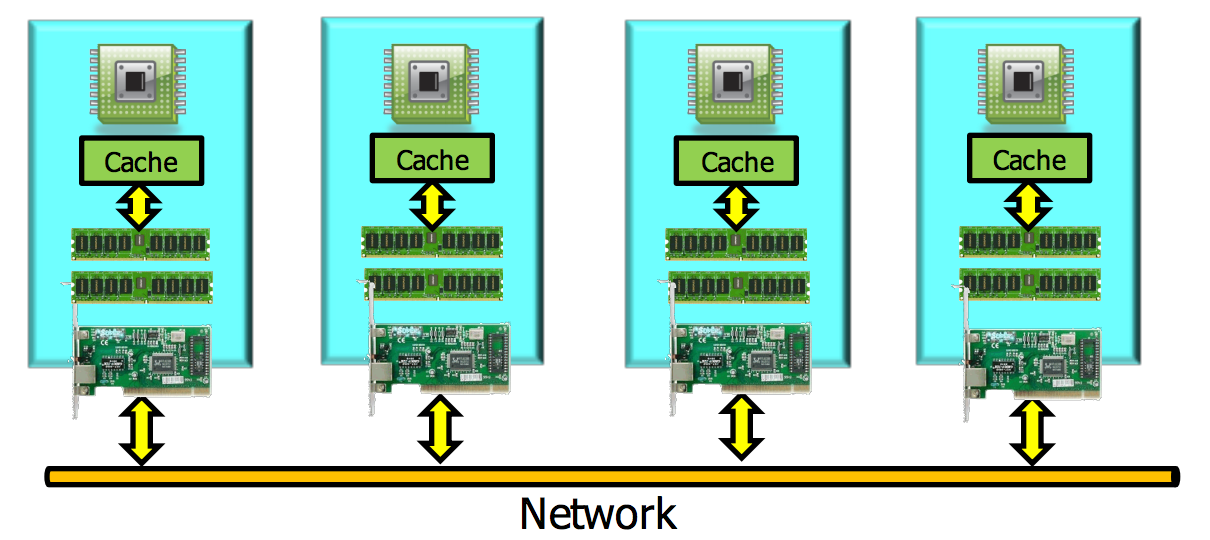
\includegraphics[width=\linewidth]{shared-nothing.png}

Wide area network : RTT (Round Trip Time) matters.. a lot !

\subsection{Fault and failure in distributed systems}

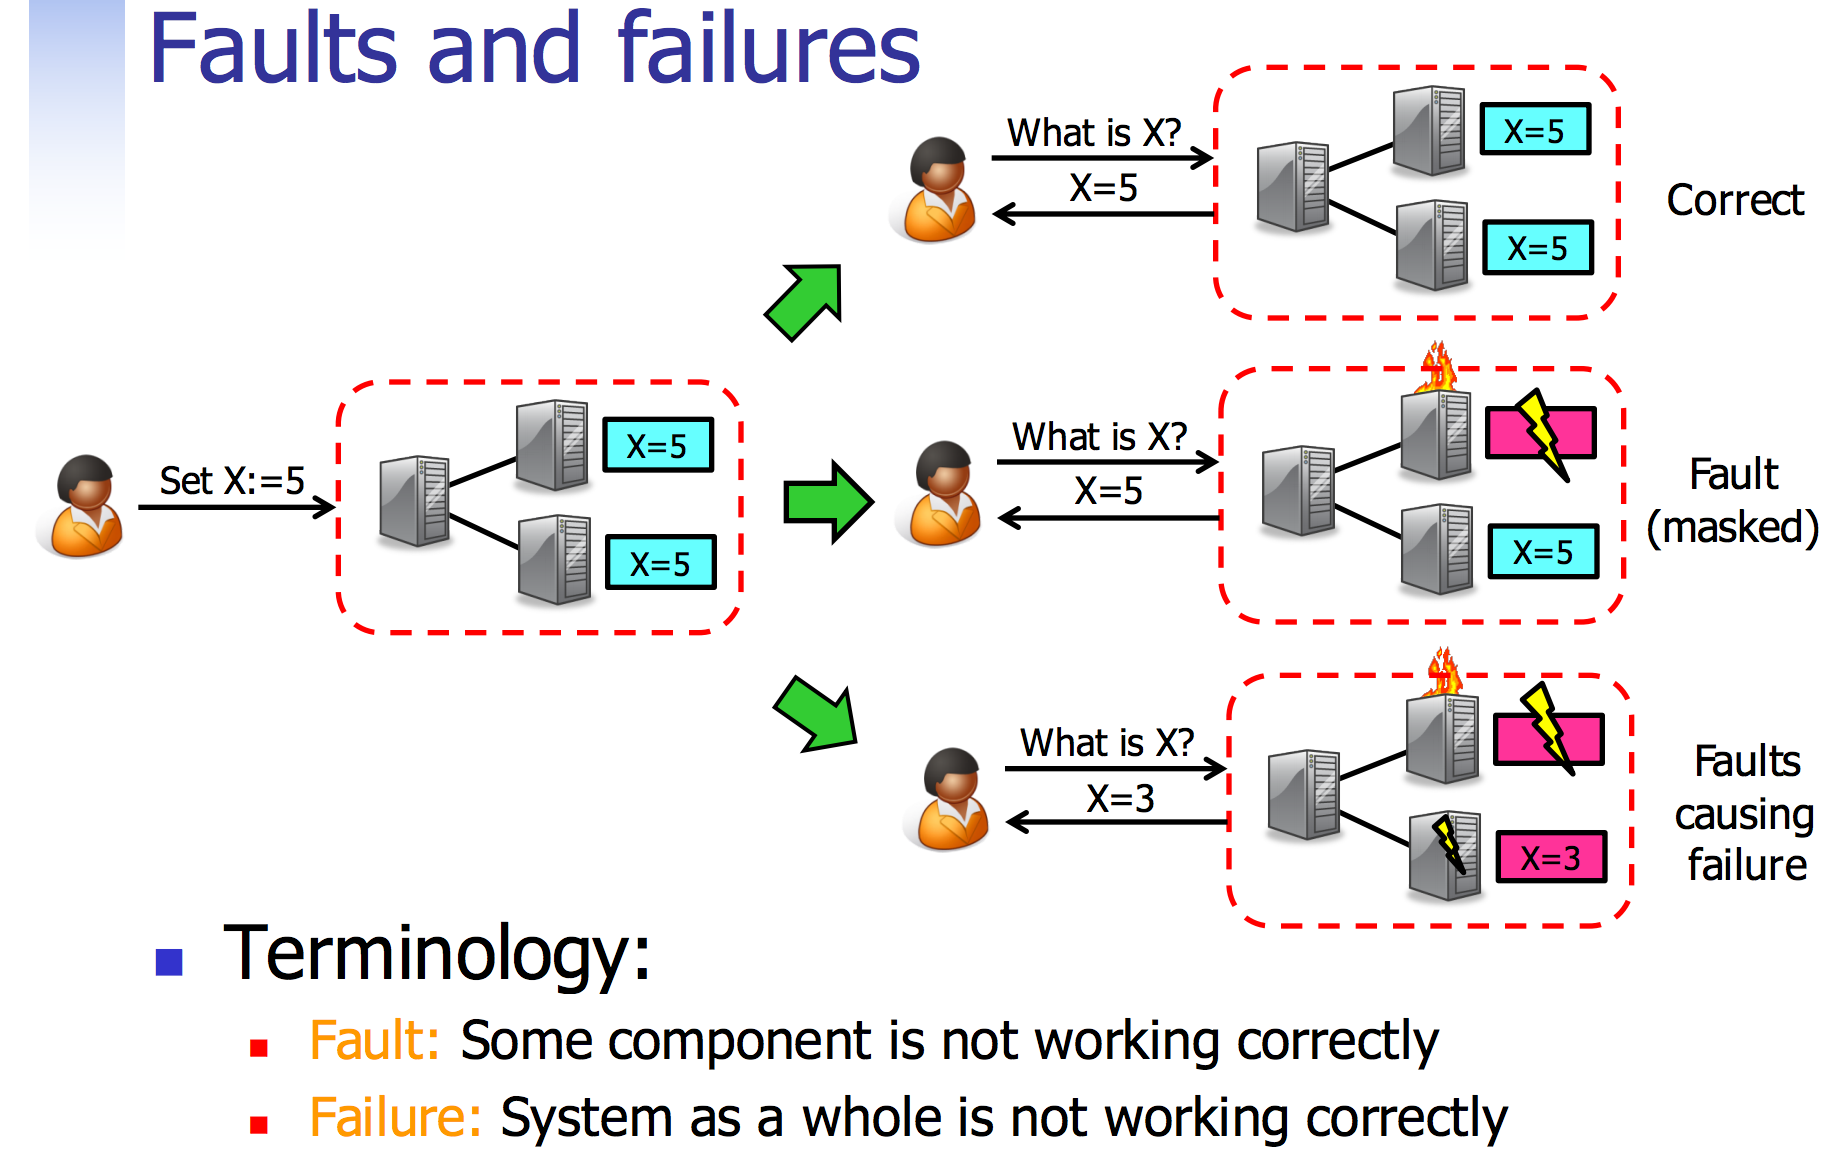
\includegraphics[width=\linewidth]{fault-fail.png}

Type of faults:
\begin{description}
\item[Crash faults] Node simply stop (OS crash, power loss)
\item[Rational behavior] Owner manipulates node to increase profit (Traffic attraction attack)
\item[Byzantine faults] Arbitrary - faulty node could do anything  (Node compromised by a hacker, compromised data, etc.)
\end{description}

A fault can lead to a domino efffect. Fault can be correlated with others.

What can be done ?
\begin{description}
\item[Prevention and avoidance]  Temporal Logic Action (formal methods are a particular kind of mathematically based techniques for the specification, development and verification of software and hardware systems)
\item[Detection] Cross-check network's route announcements with other information to see whether it is lying, and hold it accountable if it is
\item[Masking]  Store replicas of the data on multiple nodes; if data is lost or corrupted on one of them, we still have the other copies. Problem => Consistency (see before)
\item[Mitigation] 
\end{description}

\subsection{Storage system consistency: example}

We have N nodes that can store data.
To write a value: Pick W replicas and write the value to each, using a fresh timestamp
To read a value:
\begin{itemize}
\item Pick R replicas and read the value from each
\item Return the value with the highest timestamp
\item If any replicas had a lower timestamp, send them the newer value
\end{itemize}

Strong consistency :
\begin{description}
\item[Majority quorum] Always write to and read from a majority of nodes. At least one node knows the most recent value.  tolerate up to ⌈N/2⌉ - 1 crashes. But have to read/write ⌊N/2⌋ + 1 values.
\item[Read/write quorums] Read R nodes, write W nodes, s.t. R + W > N. Adjust performance of reads/writes. But availability can suffer.
\item[Consensus solutions] Paxos (for crash faults), PBFT (for Byzantine faults). Idea : Correct replicas ``outvote'' faulty ones.
\end{description}
 
The cap theorem : We can get at most two out of the three
\begin{itemize}
\item Consistency : All clients single up-to-data copy of the data, even in the presence of concurrent updates
\item Availability: Every request (including updates) received by a non-failing node in the system must result in a response, even when faults occur
\item Partition-tolerance: Consistency and availability hold even when the network partitions
\end{itemize}

Dealing with network partitions when a partition is cut : Enter an explicit partition mode that can limit some operations.


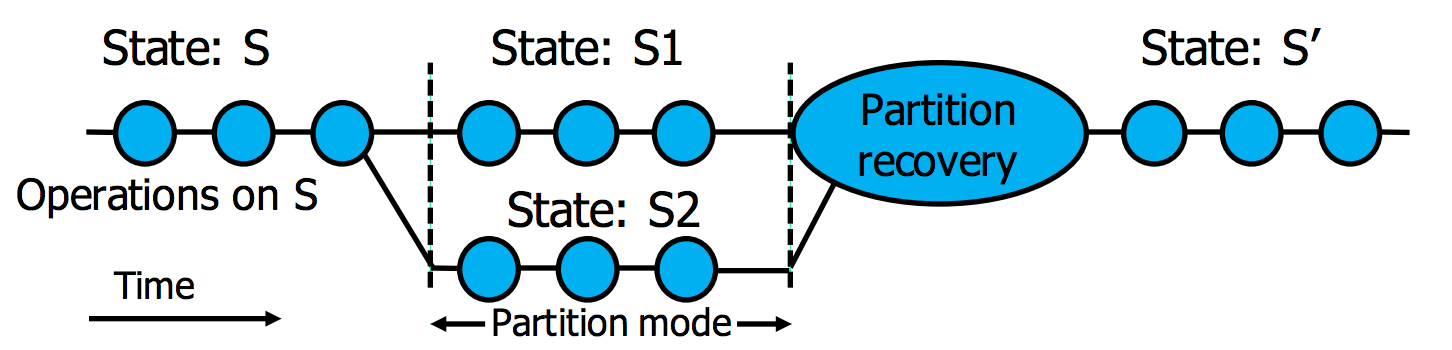
\includegraphics[width=\linewidth]{part.png}

\subsection{Relaxed consistency: ACID vs. BASE}

ACID => Atomicity, Consistency, Isolation, Durability
BASE => Basically Available, Soft-state, Eventually consistent

\subsubsection{Consistency and partitions}
=> Use replication to mask limited \# of faults
=> Partition tolerance, availability, consistency? Typically trade-off between C and A

\section{Another chapter}


\end{document}
